\section{Quand la pression diminue}

Un manomètre étant fixé à l'extrémité d'une seringue, Enzo veut étudier l'influence du volume sur la pression de l'air. Voici le relevé de ses valeurs :

\begin{center}
	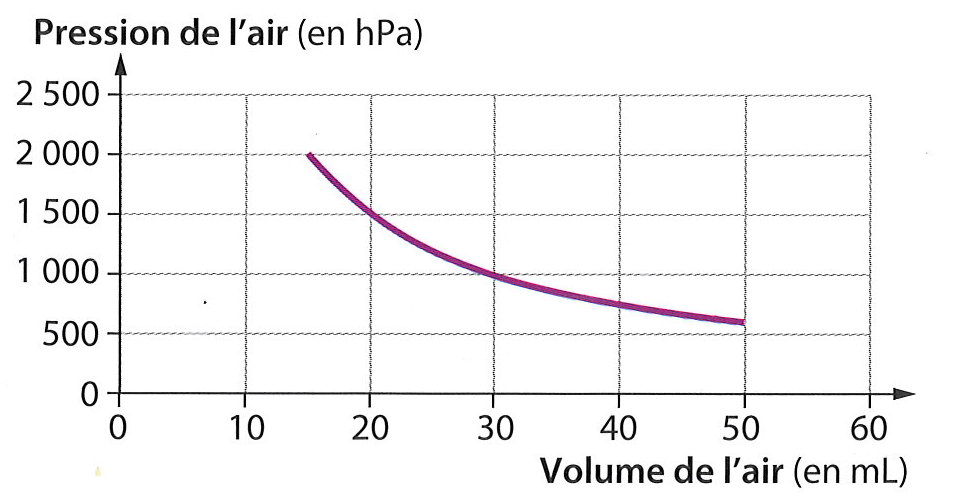
\includegraphics[scale=1.5]{pression}
\end{center}

\begin{questions}
	\question Quel est le volume d'air enfermé dans la seringue lorsqu'il est à pression atmosphérique ? ($P_{atm}=1013 hPa$)
	
	\fillwithdottedlines{2cm}
	
	\question Comment varie la masse d'air dans la seringue lorsque le volume augmente ? Justifier.
	
	
	\fillwithdottedlines{2cm}
	
	\question Comment évolue la pression de l'air enfermé dans la seringue lorsque le volume augmente ?
	
	\fillwithdottedlines{2cm}
	
	%\question La pression est-elle proportionnelle au volume d'air dans la seringue ?
	
	%\fillwithdottedlines{2cm}
	
	\question En utilisant le modèle microscopique du gaz, proposer une explication à l'évolution de la pression du gaz dans la seringue lorsque le volume augmente.
	
	\fillwithdottedlines{3cm}
\end{questions}